\documentclass[10pt,a4paper]{article}
%\usepackage[ngerman]{babel}
\usepackage{color}
\usepackage{listings}
\usepackage{graphicx}
\usepackage{float}
%\usepackage{moreverb}
\usepackage[section]{placeins}
\usepackage{hyperref}
\usepackage{algorithm}
\usepackage{algorithmicx}
\usepackage{algpseudocode}


\setlength{\parindent}{1cm} % Default is 15pt.

\title{\textbf{Shape Matching with Earth Mover's Distance}}
\author{Jon Volkmar\\
		Mart\'{i} Griera}
\date{}
\begin{document}

\maketitle

\section{Introduction}

Nowadays we have the need to solve the problem of searching for digital images in large databases. CBIR (Content-Based Image Retrieval) is the application of computer vision techniques to this image retrieval problem. Although it is relatively expensive to compute, the results it offers are often more accurate (from the human point of view) than the results of image retrieval with concept based approaches (this is, image retrieval through image meta-data like size, format, associated descriptive keywords, etc.).

Our project idea is to approach the CBIR problem with shape matching techniques, mainly using EMD (Earth Mover's Distance) as a similarity measure.
	
More concretely, we will have a database with images clustered by object class (i.e. trees, birds, cars, etc.). Our system will be able to receive a query image and try to guess its objects class, by simply computing the similarity (we will explain later how we use the EMD to measure it) between the query image and all the images in the database, and by finding in which cluster the query image has more similar images. We will work with different datasets in order to compare the results, from images that represent simple shapes in black and white to real pictures. (NOTE: object class is not currently implemented and we may use this idea of classifying images by category as a kind of evaluation metric.)

\section{Previous Work}

\section{Signature Generation}

We don't compute the EMD directly on images; first we will go over a feature extraction step to extract the more meaningful information of the images and store it as the so-called “signatures”, that are actually weighted point sets. Thus, we will have a data base of signatures, and when receiving a new query image we will generate its signature too. At this point, we will be able to calculate the EMD between the signature of the query image and all the signatures in the data base, establishing a ranking ordered by these EMDs (the lower the EMD, the more similar the signatures, and supposedly the images). Then, we will be able to answer which are the top N most similar images to the query image.

The signature generation process, inspired by the approach of logo matching \cite{panos05} is outlined in Algorithm ~\ref{alg:generateSignature}. The resulting weighted point set will be what we defined as a signature. To detect edges, corners and computation of the intensity gradient we will use a C++ library for computer vision called OpenCV (\url{http://opencv.org/}). This library also offers a function to calculate the EMD between signatures, but as there are several implementations on the web for computing it and we wanted to be able to learn, tweak and test the algorithm, we decided to use one of these implementations (\url{http://vision.stanford.edu/~rubner/emd/default.htm}).

\begin{algorithm}
\caption{Generate image signature}
\label{alg:generateSignature}
\begin{algorithmic} 
\State Find $edges$ in image using Canny edge detector  (Figure ~\ref{fig:canny})
\State Find $corners$ in image using Harris corner detector  (Figure ~\ref{fig:harris})
\State Generate X partial derivative of intensity image using Sobel operator
\State Generate Y partial derivative of intensity image using Sobel operator
\State Combine X and Y partial derivatives to form intensity gradient magnitude image  (Figure ~\ref{fig:sobel})
% \State $edges\gets $ CannyEdgeDetector($image$)
%\State $corners\gets $ HarrisCornerDetector($image$)
%\State $d_x \gets $ SobelOperatorX($image$)
%\State $d_y \gets $ SobelOperatorY($image$)
%\State $D \gets 0.5 \cdot d_x + 0.5 \cdot d_y$

%\item  Find edges in image using Canny Edge detector 
%\item Find corners in image using Harris corner detector
%\item Generate X partial derivative of intensity image using Sobel operator
%\item Generate Y partial derivative of intensity image using Sobel operator
%\item Combine X and Y partial derivatives to form intensity gradient magnitude image
%\end{itemize}
\For{$ corner$ in $corners$} 
 \If{ $corner$ is on an $edge \in edges$ }
   \State Add point of corner to point set, with weight equal to value of intensity of point on gradient image  (figure ~\ref{fig:pointset})
 \EndIf  
\EndFor

\end{algorithmic}
\end{algorithm}

\begin{figure}[ht!]
\centering
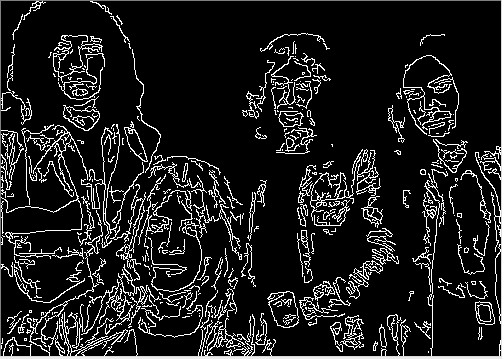
\includegraphics{canny_edge.png}
\caption{Output of Canny edge detector - edges are marked with a white outline}
\label{fig:canny}
\end{figure}

\begin{figure}[ht!]
\centering
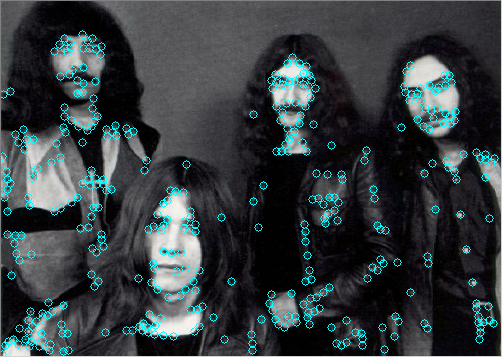
\includegraphics{harris_corner.png}
\caption{Harris Corner Detection - Detected corners are marked with blue circles}
\label{fig:harris}
\end{figure}

\begin{figure}[ht!]
\centering
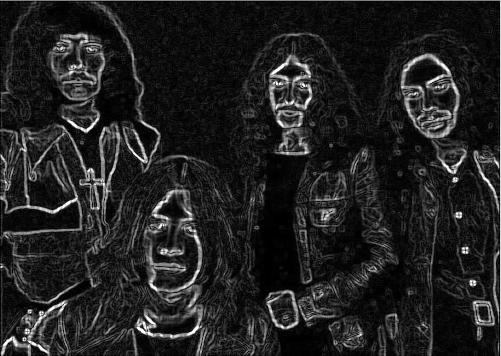
\includegraphics{sobel_intensity_gradient.png}
\caption{Image of the magnitude of the intensity gradient, calculated using the Sobel operator}
\label{fig:sobel}
\end{figure}

\begin{figure}[ht!]
\centering
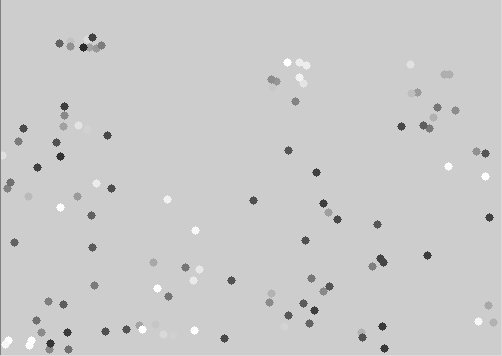
\includegraphics{weighted_point_set.png}
\caption{Each corner that is on a detected edge is given a weight, corresponding to the intensity gradient value at the same location, giving us a weighted point set. Low weights are black, high weights are white.}
\label{fig:pointset}
\end{figure}

\begin{figure}[ht!]
\centering
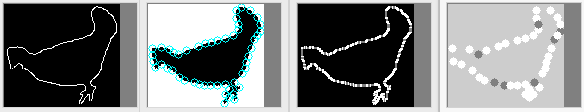
\includegraphics{bird_points.png}
\caption{Detected edges, detected corners, intensity gradient magnitude, and weighted point set for a simple shape (solid black shape on white background)}
\label{overflow}
\end{figure}

\section{Preliminary Results}

Tables ~\ref{tab:shapeQueries}~\ref{tab:buffyQueries} show the results of querying image database with images from inside the database itself. To find the nearest neighbours to the query image, we simply iterate through all images in the database and order all images by EMD value to the query image in decreasing order. The five nearest neighbors are shown, with their corresponding EMD score.

\begin{table}
    \caption{Queries on simple shape data set, 218 images \url{http://www.lems.brown.edu/vision/researchAreas/SIID/}}
    \label{tab:shapeQueries}
    \begin{tabular}{|l|l|l|l|l|l|}
        \hline
        Query image & Match 1 & Match 2 & Match 3 & Match 4 & Match 5 \\ \hline

        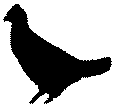
\includegraphics[width=20mm]{queries/bird09.png} &	
	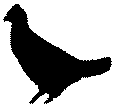
\includegraphics[width=20mm]{queries/bird09.png}  & 
	
\includegraphics[width=20mm]{queries/bird18.png}  &
	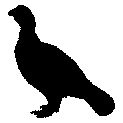
\includegraphics[width=20mm]{queries/bird07.png}  &
	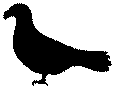
\includegraphics[width=20mm]{queries/bird19.png} &
	
\includegraphics[width=20mm]{queries/bird02.png} \\ 
	~ & 0 & 6.51677 & 7.54387 &  7.87805 & 7.87867 \\ \hline

	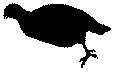
\includegraphics[width=20mm]{queries/bird04.png} &	
	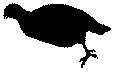
\includegraphics[width=20mm]{queries/bird04.png}  & 
	
\includegraphics[width=20mm]{queries/brick08.png}  &
	
\includegraphics[width=20mm]{queries/brick03.png}  &
	
\includegraphics[width=20mm]{queries/classic03.png} &
	
\includegraphics[width=20mm]{queries/brick04.png} \\ 
	~ & 0 & 6.53474 & 6.83729 & 6.87391 & 6.88357 \\ \hline

        \hline
    \end{tabular}
\end{table}


\begin{table}
    \caption{Queries on Buffy data set s5e6, 52 images \url{http://www.robots.ox.ac.uk/~vgg/data/buffy_pose_classes/t}}
    \label{tab:buffyQueries}
    \begin{tabular}{|l|l|l|l|l|l|}
        \hline
        Query image & Match 1 & Match 2 & Match 3 & Match 4 & Match 5 \\ \hline

        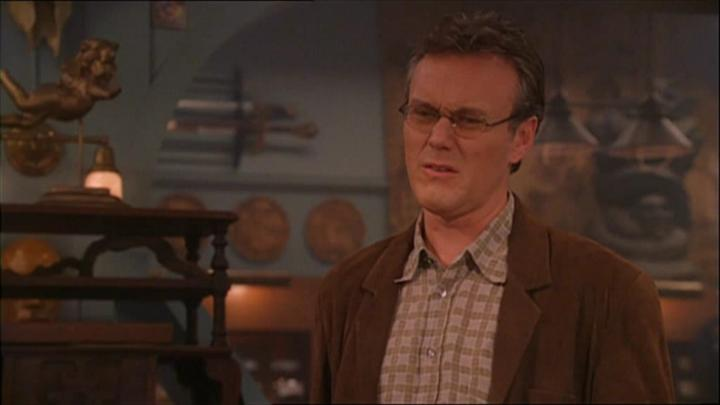
\includegraphics[width=20mm]{queries/015663.jpg} &	
	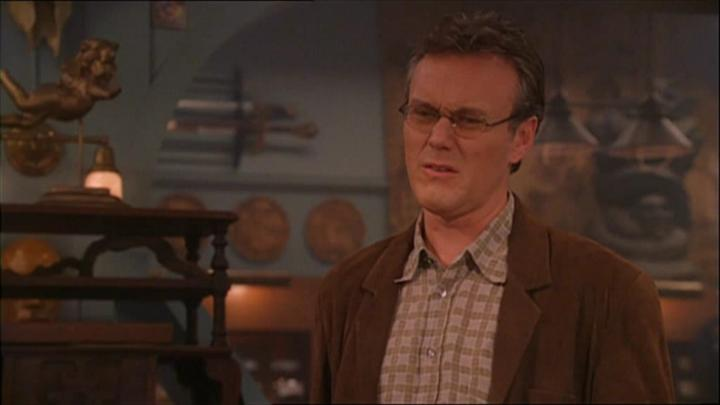
\includegraphics[width=20mm]{queries/015663.jpg} &	
	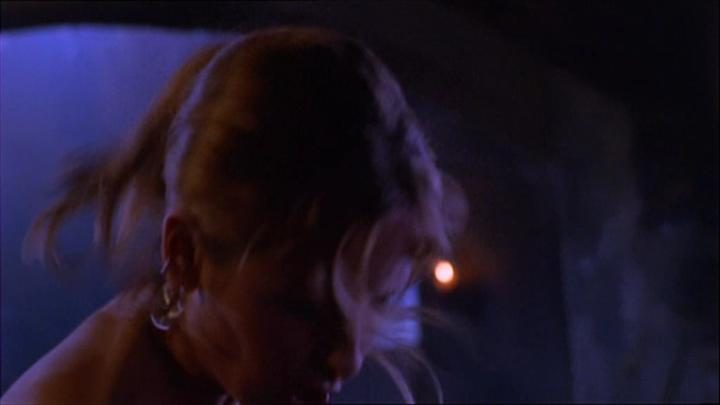
\includegraphics[width=20mm]{queries/019018.jpg}  &
	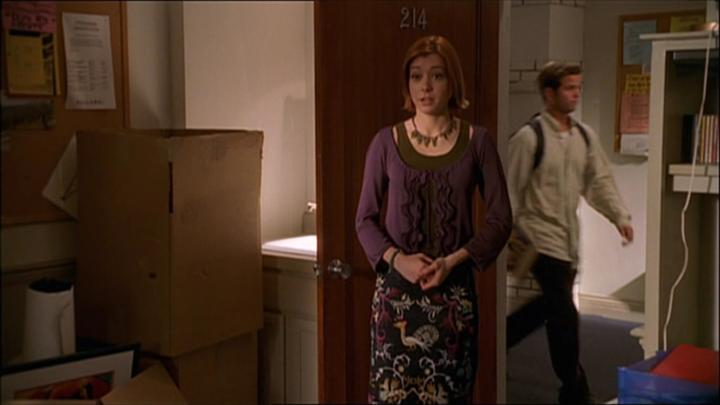
\includegraphics[width=20mm]{queries/012194.jpg}  &
	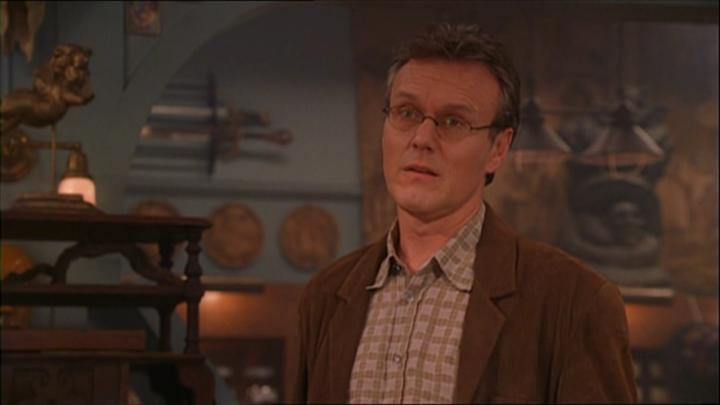
\includegraphics[width=20mm]{queries/015742.jpg} &
	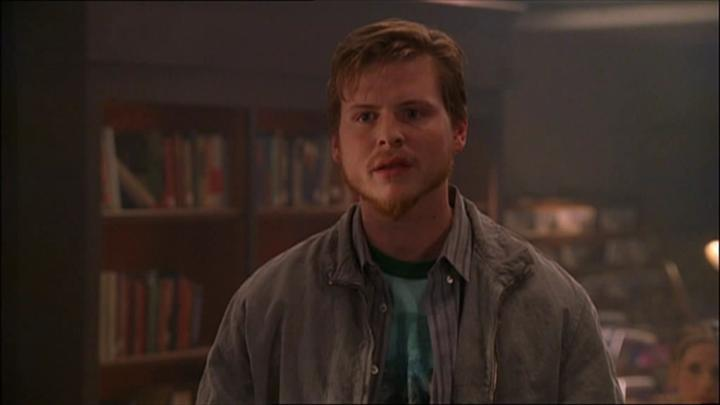
\includegraphics[width=20mm]{queries/022108.jpg} \\ 
	~ & 0 & 25.7924 & 34.351 &  37.4202 & 42.9105 \\ \hline

	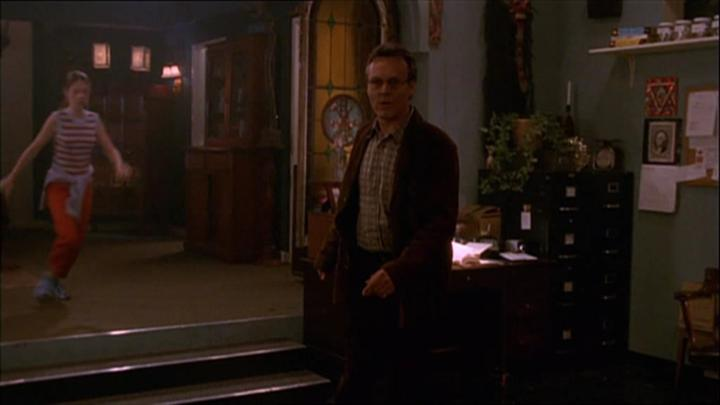
\includegraphics[width=20mm]{queries/046990.jpg} &	
	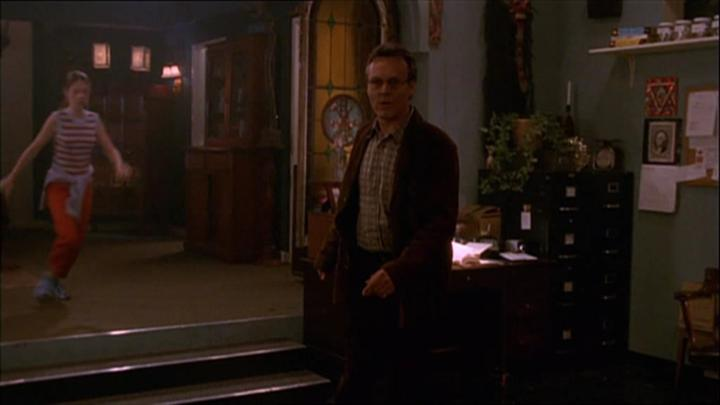
\includegraphics[width=20mm]{queries/046990.jpg}  & 
	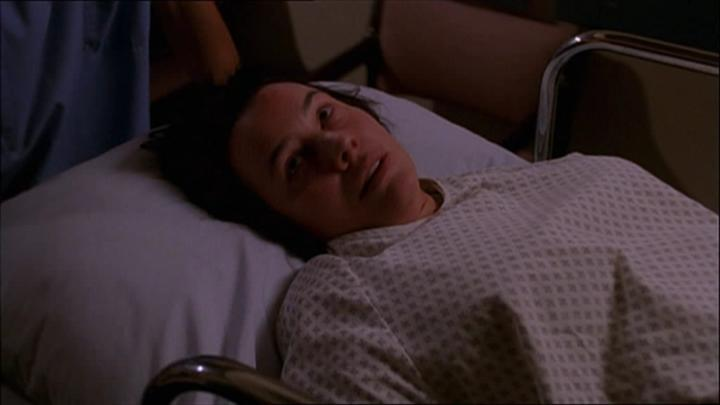
\includegraphics[width=20mm]{queries/012325.jpg}  &
	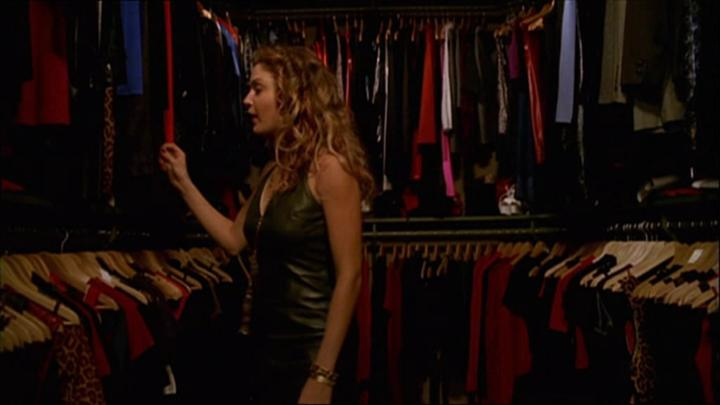
\includegraphics[width=20mm]{queries/032368.jpg}  &
	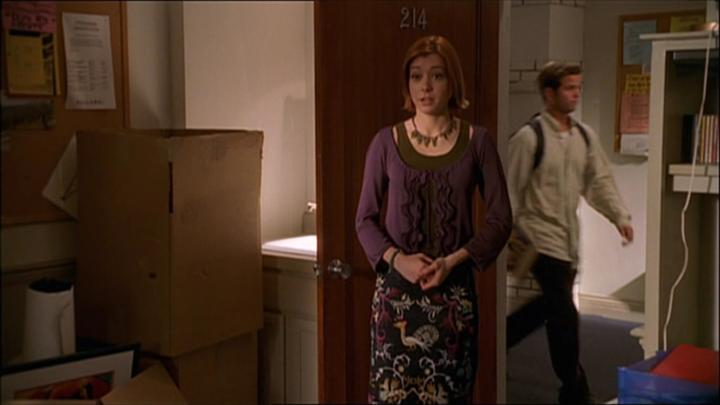
\includegraphics[width=20mm]{queries/012194.jpg} &
	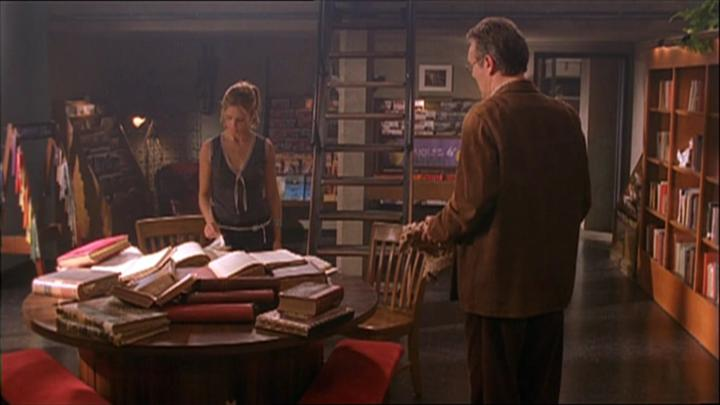
\includegraphics[width=20mm]{queries/015662.jpg} \\ 
	~ & 0 & 47 & 56.5078 & 56.8755 & 58.6826 \\ \hline

	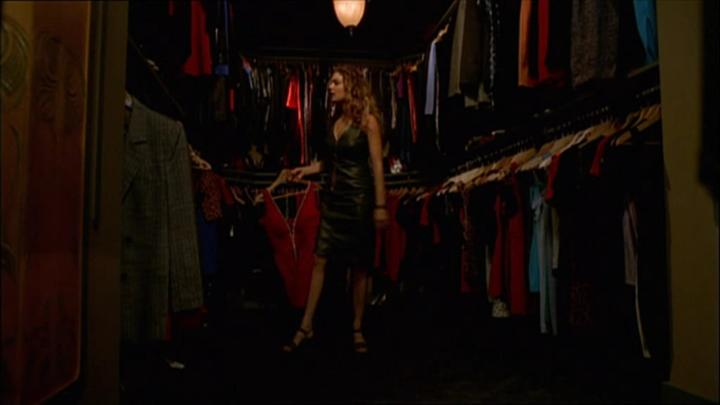
\includegraphics[width=20mm]{queries/032326.jpg} &	
	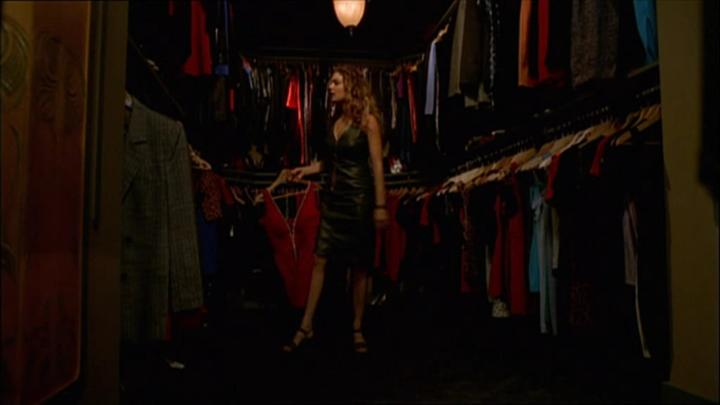
\includegraphics[width=20mm]{queries/032326.jpg}  & 
	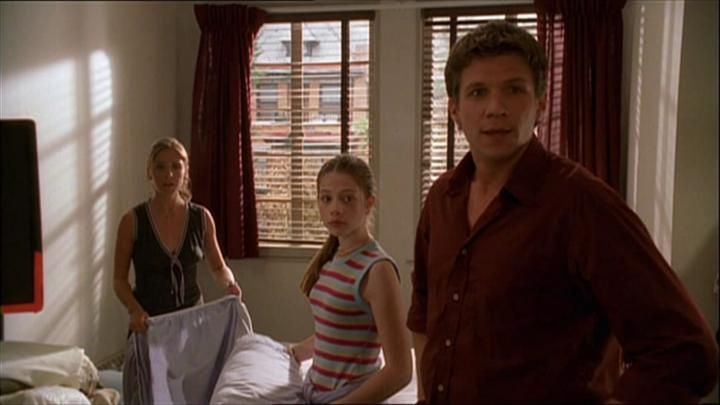
\includegraphics[width=20mm]{queries/012195.jpg}  &
	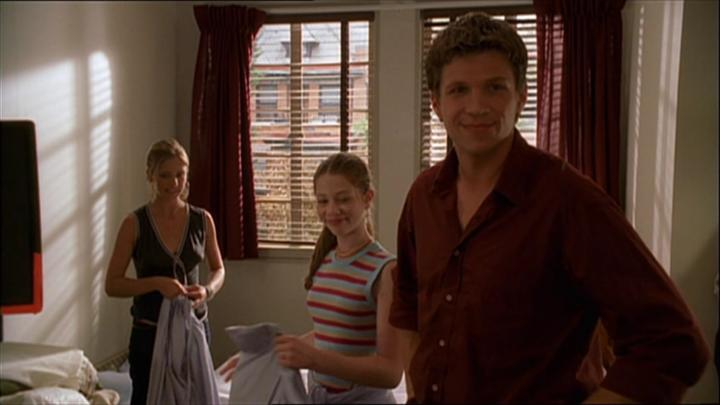
\includegraphics[width=20mm]{queries/012324.jpg}  &
	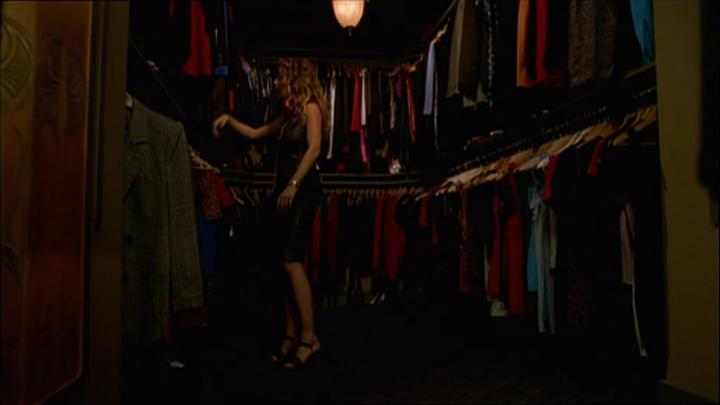
\includegraphics[width=20mm]{queries/032367.jpg} &
	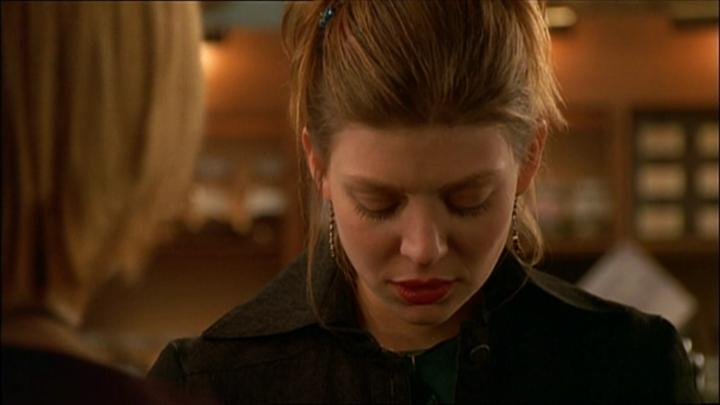
\includegraphics[width=20mm]{queries/052268.jpg} \\ 
	~ & 0 & 34.4968 & 35.6604 & 37.5272 & 42.8023 \\ \hline

        \hline
    \end{tabular}
\end{table}

\section{Further work}

The following list represents intended and possible directions to extend the existing work done in this project:

\begin{itemize}
	\item Data collection and analysis from our shape matching algorithm, and tuning of parameters
	\item Performance analysis
	\item Optimize for larger data set
	\item Build classified item database
	\item Translations, rotations, and scaling?
	\item Compare with other implementations of EMD?
	\item Other methods of generating signatures? E.g. Different kinds of features
\end{itemize}

\begin{thebibliography}{9}

\bibitem{panos05}
  P. Giannopoulous. 
  \emph{Geometric matching of weighted point sets}. 
  PhD thesis, Universiteit Utrecht, Insitute of Information and Computer Science, 2005.

\end{thebibliography}

\end{document}